\documentclass[a4paper, 11pt]{article}


%\usepackage{mathpazo}
\usepackage[onehalfspacing]{setspace}
\usepackage{graphicx}
\usepackage{amsmath, amssymb, amsfonts}
\usepackage[table]{xcolor}
\usepackage{gensymb}
\usepackage[]{booktabs}
\usepackage[utf8]{inputenc}
\usepackage{array}
\usepackage{setspace}
\usepackage{xhfill}
\usepackage{enumitem}
\usepackage{multicol}

\usepackage{geometry}
\geometry{
	total={150mm,227mm},
	left=30mm,
	top=30mm,
}

\newcommand{\cuspac}{\hspace{0.5cm}}
\newcommand{\longspac}{\hspace{1cm}}
\newcommand{\tripdot}{\cdot \cdot \cdot}
% \newcommand{\dho}{\partial} %Use this command for partial derivative command

%%%%%%%Uncomment to remove header numbering%%%%%%%%%%
%\renewcommand{\thesection}{}
%\renewcommand{\thesubsection}{}
%\renewcommand{\thesubsubsection}{}
%%%%%%%%%%%%%%%%%%%%%%%%%%%%%%%%%%%%%%%%%%%%%%%%%%%%%


\title{ADCS} %Title of Document
\date{13 April, 2023} %Date of Publishing
\author{Pranav Chandra N V\\2023AAPS0013P} %Author

\begin{document}
	\maketitle
	\newpage
	\tableofcontents
	\newpage
	
	\section{Intro}
	\begin{itemize}
		\begin{figure}[h!]
			\centering
			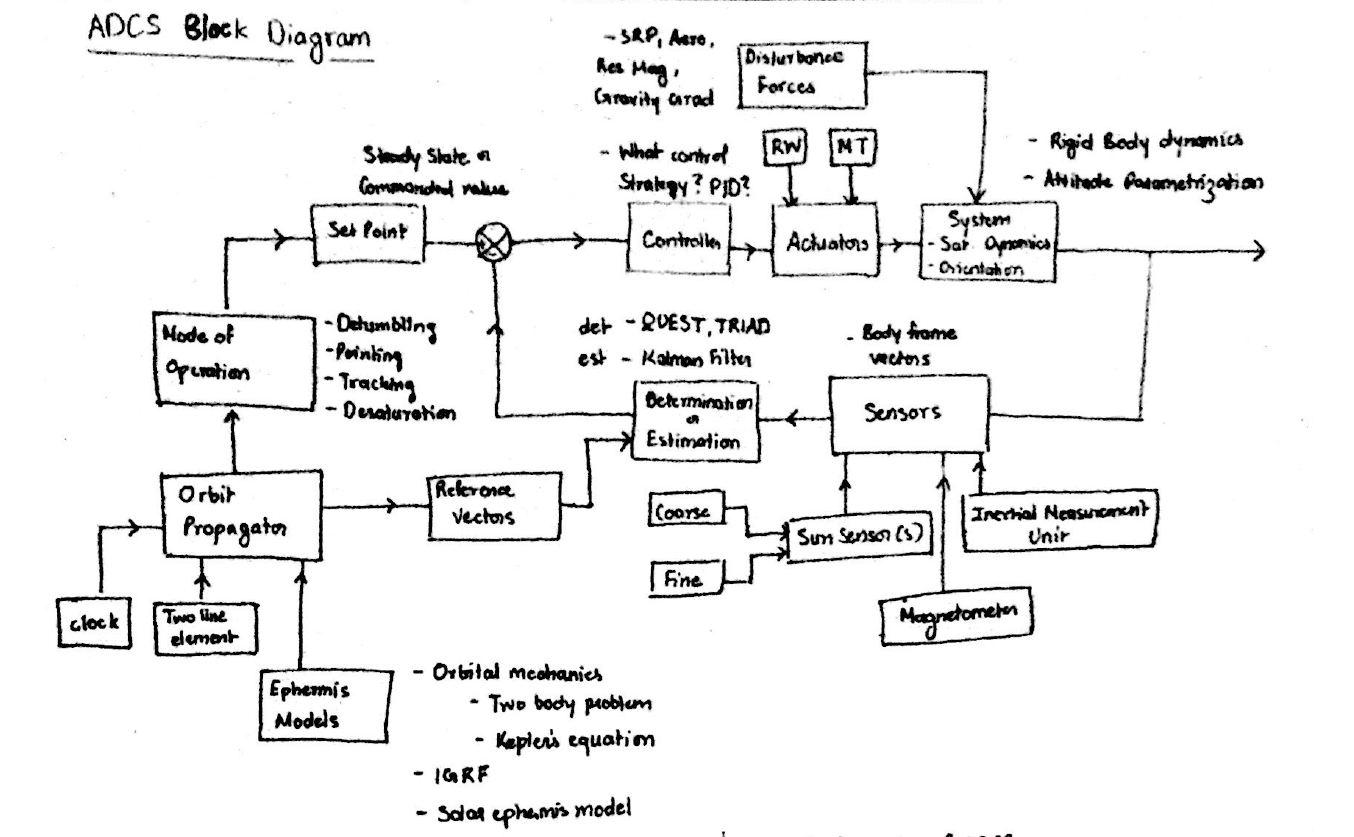
\includegraphics[scale = 0.7]{Image 1}
		\end{figure}
		\item An orbit propagator basically gives us the estimation of what the orbit will look like at any particular time.
		\item You require three things for an orbit propagator
		\begin{itemize}
			\item A clock - Required to sync things together. So that we can get the time difference between any two measurements. We take the clock directly from the OBC main clock. It's essentially a square wave.
			\item \textbf{Two line element} - Basically represents the data that comes into the system
			\begin{itemize}
				\item There are multiple forces that are experienced by the satellite. 
				\begin{itemize}
					\item Drags (caused by shape of the satellite)
					\item Winds (caused by external winds), radiation pressure (from sun and reflected from earth)
					\item Magnetic pressure (from earth's magnetic field)
					\item Gravitational force (from earth, sun, moon, etc.)
				\end{itemize}
			\end{itemize}
		\end{itemize}
		\item Modes of Operation basically comes down to two things, what modes there are and how to get into it. To check if you're pointing at the earth, you can use the series of QRs on earth.
	\end{itemize}
	
	\section{Now the (Apparently Very Basic Tensor) Math}
	\begin{itemize}
		\item A scalar is just a one dimensional vector, and are never dependent on your refrence frame. I.e. they're invariants. and a vector 
		\item When a transformation occurs, vectors transform exactly with the transformation.
		
	\end{itemize}
\end{document}
